\begin{section}
    {Tree}

\subsection*{Definition}
A tree is collection of nodes and edges. with one node distinguished as a root, along with parenthood relation, one edge connects two nodes.
Each node in the tree can be connected to many children, but must be connected to exactly one parent, except for the root node.
No cycles or loops

\bigskip\textbf{Recursive Definition} \\
Starts with a single node, then we can build a new tree by making other tress as subtrees of the single node.
\begin{center}
    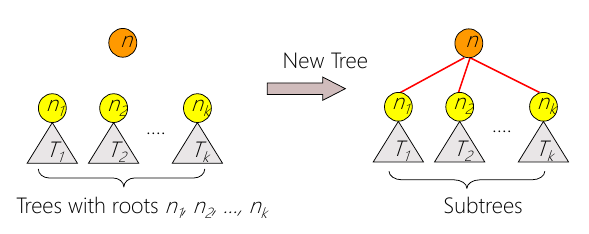
\includegraphics[]{img/treerecursivedef.png}
\end{center}

Some keywords : Parent/child, Ancestor/descendant, Siblings, Leaf, Depth, Height, Level.

\bigskip\noindent
\textbf{Binary Tree} : Every node has at most two children, Each child is designated as left child or a right child. (left child and right child are distict.)

\noindent
\textbf{Proper Tree} : Every node has 0 or 2 children.

\noindent
\textbf{Full Tree} : If it has a maximum number of nodes at each level. A full binary tree of height h has $2^{h+1} - 1$ nodes.
\bigskip

Node numbering :
\begin{enumerate}
    \item Zero-based numbering: \\
    \begin{tabular}{|c|c|c|c|c|c|c|c|c|c|}
        \hline
        \textbf{Array} & 0 & 1 & 2 & 3 & 4 & 5 & 6 & 7 & ... \\
        \hline
    \end{tabular}
    
    \bigskip\noindent
    Node 0 is the root, and the left child of node i is 2i+1, and the right child of node i is 2i+2. Parent node is $\lfloor \frac{i-1}{2} \rfloor$.
    \item One-based numbering: \\
    \begin{tabular}{|c|c|c|c|c|c|c|c|c|c|}
        \hline
        \textbf{Array} & 1 & 2 & 3 & 4 & 5 & 6 & 7 & 8 & ... \\
        \hline
    \end{tabular}

    \bigskip\noindent
    Node 1 is the root, and the left child of node i is 2i, and the right child of node i is 2i+1. Parent node is $\lfloor \frac{i}{2} \rfloor$.
\end{enumerate}

\noindent\textbf{Complete Binary Tree} : Relaxed definition of a full binary tree. A binary tree of height h is complete, if all levels possibly except h are completely full, and level h is filled from left to right.

\bigskip\noindent
\textbf{implementation}
\begin{itemize}
    \item Array implementation : Node numbered k is stored in an array tree[k].
    \item Linked Implementation : Struct Node {value, left, right}
\end{itemize}

\subsubsection*{Tree Traversal}

Tree traversal is passing through the tree and visiting each node exactly once (linearization). There are three ways to traverse the tree. (preorder, inorder, postorder). All of tree traversal is variant of depth-first search(DFS) complemented by  or recursive function call. Exceptionally, level-order traversal is breadth-first search(BFS) complemented by queue.
\begin{itemize}
    \item Preorder(T) = \textless n, Preorder($T_1$), Preorder($T_2$), ..., Preorder($T_k$)\textgreater
    \item Inorder(T) = \textless Inorder($T_1$), n, Inorder($T_2$), ..., Inorder($T_k$)\textgreater
    \item Postorder(T) = \textless Postorder($T_1$), Postorder($T_2$), ..., Postorder($T_k$), n\textgreater
\end{itemize}

\noindent Two type of traversal :
\begin{itemize}
    \item Depth-first traversal \\
    Go down first, recursive way, 3 variation : preorder, inorder, postorder
    \item Breadth-first traversal \\
    Go across first in same level, No variation, just level-order traversal
\end{itemize}

\noindent
For getting Unique binary tree by two traversals, only 3 types are valid : \textbf{(postorder and inorder), (preorder and inorder), (levelorder and inorder)}. 
Inorder are necessary to find left and right child, and postorder/preorder/levelorder are necessary to find root.

\bigskip
Some type of general tree implementations. This is example. 
\medskip
\textbf{Simple Approach} \\
\textbf{List-of-Children Approach} \\
\textbf{Left-Child/Right-Sibling Approach} \\
\textbf{TODO}
% //TODO ---



\subsubsection*{Converting into a Binary Tree : Donald Knuth}
Input : general trees. Then leftmost child is left child, and right sibling is right child. Finally, remove the other links. It seems like rotating the tree clockwise by 45$\deg$. When going from parent to leftchild, level be increase by 1 from original tree, and when going from parent to rightchild, level be same as original tree. Preorder is same, Postorder of original will be Inorder of new binary tree.


\bigskip
\end{section}